%%*************************************************************************
%% Legal Notice:
%% This code is offered as-is without any warranty either expressed or
%% implied; without even the implied warranty of MERCHANTABILITY or
%% FITNESS FOR A PARTICULAR PURPOSE! 
%% User assumes all risk.
%% In no event shall IEEE or any contributor to this code be liable for
%% any damages or losses, including, but not limited to, incidental,
%% consequential, or any other damages, resulting from the use or misuse
%% of any information contained here.
%%
%% All comments are the opinions of their respective authors and are not
%% necessarily endorsed by the IEEE.
%%
%% This work is distributed under the LaTeX Project Public License (LPPL)
%% ( http://www.latex-project.org/ ) version 1.3, and may be freely used,
%% distributed and modified. A copy of the LPPL, version 1.3, is included
%% in the base LaTeX documentation of all distributions of LaTeX released
%% 2003/12/01 or later.
%% Retain all contribution notices and credits.
%% ** Modified files should be clearly indicated as such, including  **
%% ** renaming them and changing author support contact information. **
%%
%% File list of work: IEEEtran.cls, IEEEtran_HOWTO.pdf, bare_adv.tex,
%%                    bare_conf.tex, bare_jrnl.tex, bare_jrnl_compsoc.tex
%%*************************************************************************

% Note that the a4paper option is mainly intended so that authors in
% countries using A4 can easily print to A4 and see how their papers will
% look in print - the typesetting of the document will not typically be
% affected with changes in paper size (but the bottom and side margins will).
% Use the testflow package mentioned above to verify correct handling of
% both paper sizes by the user's LaTeX system.
%
% Also note that the "draftcls" or "draftclsnofoot", not "draft", option
% should be used if it is desired that the figures are to be displayed in
% draft mode.
%
\documentclass[conference]{IEEEtran}

% *** MISC UTILITY PACKAGES ***
%
\usepackage{ifpdf}
% Heiko Oberdiek's ifpdf.sty is very useful if you need conditional
% compilation based on whether the output is pdf or dvi.
% usage:
% \ifpdf
%   % pdf code
% \else
%   % dvi code
% \fi
% The latest version of ifpdf.sty can be obtained from:
% http://www.ctan.org/tex-archive/macros/latex/contrib/oberdiek/
% Also, note that IEEEtran.cls V1.7 and later provides a builtin
% \ifCLASSINFOpdf conditional that works the same way.
% When switching from latex to pdflatex and vice-versa, the compiler may
% have to be run twice to clear warning/error messages.

\usepackage{blindtext}
\usepackage{placeins}
\usepackage{graphicx}
\usepackage{epstopdf}

% use color package to make todos jump out in text
\usepackage{color}
% macro for todo entries addition
\newcommand{\addtodo}[1]{\textcolor{red}{[[#1]]}}

\definecolor{light-gray}{gray}{0.75}
\newcommand{\dummytext}{\textcolor{light-gray}{\Blindtext}}


% *** CITATION PACKAGES ***
%
%\usepackage{cite}
% cite.sty was written by Donald Arseneau
% V1.6 and later of IEEEtran pre-defines the format of the cite.sty package
% \cite{} output to follow that of IEEE. Loading the cite package will
% result in citation numbers being automatically sorted and properly
% "compressed/ranged". e.g., [1], [9], [2], [7], [5], [6] without using
% cite.sty will become [1], [2], [5]--[7], [9] using cite.sty. cite.sty's
% \cite will automatically add leading space, if needed. Use cite.sty's
% noadjust option (cite.sty V3.8 and later) if you want to turn this off.
% cite.sty is already installed on most LaTeX systems. Be sure and use
% version 4.0 (2003-05-27) and later if using hyperref.sty. cite.sty does
% not currently provide for hyperlinked citations.
% The latest version can be obtained at:
% http://www.ctan.org/tex-archive/macros/latex/contrib/cite/
% The documentation is contained in the cite.sty file itself.






% *** GRAPHICS RELATED PACKAGES ***
%
\ifpdf
  % \usepackage[pdftex]{graphicx}
  % declare the path(s) where your graphic files are
  % \graphicspath{{../pdf/}{../jpeg/}}
  % and their extensions so you won't have to specify these with
  % every instance of \includegraphics
  % \DeclareGraphicsExtensions{.pdf,.jpeg,.png}
\else
  % or other class option (dvipsone, dvipdf, if not using dvips). graphicx
  % will default to the driver specified in the system graphics.cfg if no
  % driver is specified.
  % \usepackage[dvips]{graphicx}
  % declare the path(s) where your graphic files are
  % \graphicspath{{../eps/}}
  % and their extensions so you won't have to specify these with
  % every instance of \includegraphics
  % \DeclareGraphicsExtensions{.eps}
\fi
% graphicx was written by David Carlisle and Sebastian Rahtz. It is
% required if you want graphics, photos, etc. graphicx.sty is already
% installed on most LaTeX systems. The latest version and documentation can
% be obtained at: 
% http://www.ctan.org/tex-archive/macros/latex/required/graphics/
% Another good source of documentation is "Using Imported Graphics in
% LaTeX2e" by Keith Reckdahl which can be found as epslatex.ps or
% epslatex.pdf at: http://www.ctan.org/tex-archive/info/
%
% latex, and pdflatex in dvi mode, support graphics in encapsulated
% postscript (.eps) format. pdflatex in pdf mode supports graphics
% in .pdf, .jpeg, .png and .mps (metapost) formats. Users should ensure
% that all non-photo figures use a vector format (.eps, .pdf, .mps) and
% not a bitmapped formats (.jpeg, .png). IEEE frowns on bitmapped formats
% which can result in "jaggedy"/blurry rendering of lines and letters as
% well as large increases in file sizes.
%
% You can find documentation about the pdfTeX application at:
% http://www.tug.org/applications/pdftex





% *** MATH PACKAGES ***
%
%\usepackage[cmex10]{amsmath}
% A popular package from the American Mathematical Society that provides
% many useful and powerful commands for dealing with mathematics. If using
% it, be sure to load this package with the cmex10 option to ensure that
% only type 1 fonts will utilized at all point sizes. Without this option,
% it is possible that some math symbols, particularly those within
% footnotes, will be rendered in bitmap form which will result in a
% document that can not be IEEE Xplore compliant!
%
% Also, note that the amsmath package sets \interdisplaylinepenalty to 10000
% thus preventing page breaks from occurring within multiline equations. Use:
%\interdisplaylinepenalty=2500
% after loading amsmath to restore such page breaks as IEEEtran.cls normally
% does. amsmath.sty is already installed on most LaTeX systems. The latest
% version and documentation can be obtained at:
% http://www.ctan.org/tex-archive/macros/latex/required/amslatex/math/





% *** SPECIALIZED LIST PACKAGES ***
%
%\usepackage{algorithmic}
% algorithmic.sty was written by Peter Williams and Rogerio Brito.
% This package provides an algorithmic environment fo describing algorithms.
% You can use the algorithmic environment in-text or within a figure
% environment to provide for a floating algorithm. Do NOT use the algorithm
% floating environment provided by algorithm.sty (by the same authors) or
% algorithm2e.sty (by Christophe Fiorio) as IEEE does not use dedicated
% algorithm float types and packages that provide these will not provide
% correct IEEE style captions. The latest version and documentation of
% algorithmic.sty can be obtained at:
% http://www.ctan.org/tex-archive/macros/latex/contrib/algorithms/
% There is also a support site at:
% http://algorithms.berlios.de/index.html
% Also of interest may be the (relatively newer and more customizable)
% algorithmicx.sty package by Szasz Janos:
% http://www.ctan.org/tex-archive/macros/latex/contrib/algorithmicx/




% *** ALIGNMENT PACKAGES ***
%
%\usepackage{array}
% Frank Mittelbach's and David Carlisle's array.sty patches and improves
% the standard LaTeX2e array and tabular environments to provide better
% appearance and additional user controls. As the default LaTeX2e table
% generation code is lacking to the point of almost being broken with
% respect to the quality of the end results, all users are strongly
% advised to use an enhanced (at the very least that provided by array.sty)
% set of table tools. array.sty is already installed on most systems. The
% latest version and documentation can be obtained at:
% http://www.ctan.org/tex-archive/macros/latex/required/tools/


%\usepackage{mdwmath}
%\usepackage{mdwtab}
% Also highly recommended is Mark Wooding's extremely powerful MDW tools,
% especially mdwmath.sty and mdwtab.sty which are used to format equations
% and tables, respectively. The MDWtools set is already installed on most
% LaTeX systems. The lastest version and documentation is available at:
% http://www.ctan.org/tex-archive/macros/latex/contrib/mdwtools/


% IEEEtran contains the IEEEeqnarray family of commands that can be used to
% generate multiline equations as well as matrices, tables, etc., of high
% quality.


%\usepackage{eqparbox}
% Also of notable interest is Scott Pakin's eqparbox package for creating
% (automatically sized) equal width boxes - aka "natural width parboxes".
% Available at:
% http://www.ctan.org/tex-archive/macros/latex/contrib/eqparbox/





% *** SUBFIGURE PACKAGES ***
%\usepackage[tight,footnotesize]{subfigure}
% subfigure.sty was written by Steven Douglas Cochran. This package makes it
% easy to put subfigures in your figures. e.g., "Figure 1a and 1b". For IEEE
% work, it is a good idea to load it with the tight package option to reduce
% the amount of white space around the subfigures. subfigure.sty is already
% installed on most LaTeX systems. The latest version and documentation can
% be obtained at:
% http://www.ctan.org/tex-archive/obsolete/macros/latex/contrib/subfigure/
% subfigure.sty has been superceeded by subfig.sty.



%\usepackage[caption=false]{caption}
%\usepackage[font=footnotesize]{subfig}
% subfig.sty, also written by Steven Douglas Cochran, is the modern
% replacement for subfigure.sty. However, subfig.sty requires and
% automatically loads Axel Sommerfeldt's caption.sty which will override
% IEEEtran.cls handling of captions and this will result in nonIEEE style
% figure/table captions. To prevent this problem, be sure and preload
% caption.sty with its "caption=false" package option. This is will preserve
% IEEEtran.cls handing of captions. Version 1.3 (2005/06/28) and later 
% (recommended due to many improvements over 1.2) of subfig.sty supports
% the caption=false option directly:
%\usepackage[caption=false,font=footnotesize]{subfig}
%
% The latest version and documentation can be obtained at:
% http://www.ctan.org/tex-archive/macros/latex/contrib/subfig/
% The latest version and documentation of caption.sty can be obtained at:
% http://www.ctan.org/tex-archive/macros/latex/contrib/caption/




% *** FLOAT PACKAGES ***
%
%\usepackage{fixltx2e}
% fixltx2e, the successor to the earlier fix2col.sty, was written by
% Frank Mittelbach and David Carlisle. This package corrects a few problems
% in the LaTeX2e kernel, the most notable of which is that in current
% LaTeX2e releases, the ordering of single and double column floats is not
% guaranteed to be preserved. Thus, an unpatched LaTeX2e can allow a
% single column figure to be placed prior to an earlier double column
% figure. The latest version and documentation can be found at:
% http://www.ctan.org/tex-archive/macros/latex/base/



%\usepackage{stfloats}
% stfloats.sty was written by Sigitas Tolusis. This package gives LaTeX2e
% the ability to do double column floats at the bottom of the page as well
% as the top. (e.g., "\begin{figure*}[!b]" is not normally possible in
% LaTeX2e). It also provides a command:
%\fnbelowfloat
% to enable the placement of footnotes below bottom floats (the standard
% LaTeX2e kernel puts them above bottom floats). This is an invasive package
% which rewrites many portions of the LaTeX2e float routines. It may not work
% with other packages that modify the LaTeX2e float routines. The latest
% version and documentation can be obtained at:
% http://www.ctan.org/tex-archive/macros/latex/contrib/sttools/
% Documentation is contained in the stfloats.sty comments as well as in the
% presfull.pdf file. Do not use the stfloats baselinefloat ability as IEEE
% does not allow \baselineskip to stretch. Authors submitting work to the
% IEEE should note that IEEE rarely uses double column equations and
% that authors should try to avoid such use. Do not be tempted to use the
% cuted.sty or midfloat.sty packages (also by Sigitas Tolusis) as IEEE does
% not format its papers in such ways.





% *** PDF, URL AND HYPERLINK PACKAGES ***
%
%\usepackage{url}
% url.sty was written by Donald Arseneau. It provides better support for
% handling and breaking URLs. url.sty is already installed on most LaTeX
% systems. The latest version can be obtained at:
% http://www.ctan.org/tex-archive/macros/latex/contrib/misc/
% Read the url.sty source comments for usage information. Basically,
% \url{my_url_here}.





% *** Do not adjust lengths that control margins, column widths, etc. ***
% *** Do not use packages that alter fonts (such as pslatex).         ***
% There should be no need to do such things with IEEEtran.cls V1.6 and later.
% (Unless specifically asked to do so by the journal or conference you plan
% to submit to, of course. )


% correct bad hyphenation here
\hyphenation{op-tical net-works semi-conduc-tor}


\begin{document}
%
% paper title
% can use linebreaks \\ within to get better formatting as desired
\title{\textbf{Dfuzzer: A D-Bus fuzzing tool}\addtodo{Better title? It's a
fuzzer for D-Bus using applications}}

% author names and affiliations
% use a multiple column layout for up to three different
% affiliations
\author{\IEEEauthorblockN{Mat\'{u}\v{s} Marfefka and Petr Muller,}
\IEEEauthorblockA{Faculty of Information Technology\\
Brno University of Technology,\\
Bo\v{z}et\v{e}chova 1/2 Brno, Czech Republic}
\IEEEauthorblockA{Red Hat,\\
Purky\v{n}ova 99/75a Brno, Czech Republic}
\addtodo{Fix typesetting. How to typeset double affiliations?}
}
% conference papers do not typically use \thanks and this command
% is locked out in conference mode. If really needed, such as for
% the acknowledgment of grants, issue a \IEEEoverridecommandlockouts
% after \documentclass

% make the title area
\maketitle


\begin{abstract}
\addtodo{Use the special caps for Dfuzzer name, and possibly others}
We present Dfuzzer, a fully automated tool for fuzz testing
programs communicating via D-Bus, the prevalent modern mechanism for an
inter-process communication in GNU/Linux ecosystem. With the GNU/Linux systems
generally going towards tighter and better integrated systems, even the basic
building stones of the operating systems start using D-Bus for communication,
like systemd, the modern GNU/Linux system and service manager. With these
important programs receiving data over D-Bus, it is important that they
sanitize the inputs correctly. Unfortunately, it is often not the case, as
demonstrated by serious bugs found by our fuzzing tool.

Dfuzzer is fully automated: using D-Bus introspection, it is able to acquire
the structure of the data the target program expects, and generate ballast
data respecting this structure, so the target program starts using them
incorrectly if it does not carefully validate it. We have found numerous bugs
in various parts of the GNU/Linux operating system, including Gnome Shell and
systemd. The bugs usually result in crashes, but we have found even some
security sensitive issues as well as data-loss bugs.

In this paper, we briefly describe the eco-system related to D-Bus. We follow
with the description of the tool. In the end, we present the application of the
tool for the systematic testing of various operating system parts, and show the
most interesting bugs we have found. We also discuss the software engineering
aspects of fuzz testing D-Bus: we have met developer's opinions that the
problems found do not constitute a valid bugs, because the D-Bus interface is
actually an internal API. The discussion is interesting by showing that the
D-Bus usage is not a fully mature area of engineering, and the programmers do
not have a shared understanding of its purpose.
\addtodo{The abstract is very long. Prune?}
\addtodo{Re-check after finishing the text}
\end{abstract}

\begin{keywords}
D-Bus, fuzzer, fuzz testing, automation, pseudo-random data generation, IPC
\end{keywords}

% For peer review papers, you can put extra information on the cover
% page as needed:
% \ifCLASSOPTIONpeerreview
% \begin{center} \bfseries EDICS Category: 3-BBND \end{center}
% \fi
%
% For peerreview papers, this IEEEtran command inserts a page break and
% creates the second title. It will be ignored for other modes.
\IEEEpeerreviewmaketitle



\section{Introduction}
D-Bus is a~binary protocol and~a~message bus system providing applications
a~simple way to~talk to~one another. D-Bus is ``\emph{a~system for~\mbox{inter-process}
communication~(IPC) and~Remote Procedure Calling~(RPC) between
processes running on the same machine and~makes it simple and~reliable to~code
a~`single instance' application or daemon, and~to~launch applications and~daemons
on~demand when their services are needed}''~\cite{DBUS}.

Recently, D-Bus has become important part of~almost all GNU/Linux
distributions. There are more and~more applications which use it for~IPC,
including key system parts like service managers. The growing importance is witnessed
by the recent inclusion of the D-Bus message bus directly into the Linux kernel
upstream.

Applications communicating via D-Bus either provide interfaces which contain callable
methods with~input arguments, or call such methods over
the message bus, providing arguments for them. This means the programs
receiving the data must carefully validate it, because they may originate in
any program having access to the message bus. Unfortunately, this does not seem
to be the usual case, and programs rely on convention and good will of the
callers.

This structure means the D-Bus communicating programs are a good target for
fuzz testing, which is well-suited for detecting bugs stemming from improper
validation of input data. Fuzz testing (or simply fuzzing) is a~well-known type
of~testing\cite{Fuzzing2, Fuzzing}: it it an automated, brute force, black-box
technique, exploiting the~fact that many bugs in~software are caused
by~handling inputs without applying proper validation routines on~those.
Fuzzing is close to~the~boundary value analysis, where you create test values
that infringe the~boundary of~known good and~bad values.  Fuzz testing has a
long history of being applied in security area \addtodo{citations!}, because
the type of bugs it finds often has security implications: improper validation
sometimes means there is a possibility to carefully craft the input so the
program does something useful to the attacker. Outside the security testing
domain, the technique was successfuly used for finding bugs in
compilers\addtodo{cite}.

The advantage of fuzz testing is that the bug detection is easily automated: in
the most basic form, the tool can just send random data as the input of the
program, and the program should not misbehave (usually, crash), but handle the
wrong input gracefully. Specific application of the technique improve efficiency by
carefully crafting the input so it adheres to the protocol expected by the
program, but having random semantics, so it passes the basic validation and
penetrates deeper into the program. For example, if a program expects XML as an
input, the fuzzer will not generate random data, as that would be refused by
the most basic XML parser. Instead, a valid XML containing random elements and
their content is generated, to see how the program validates the input beyond
it simply being an XML.

\section{DBus message bus}
\addtodo{Trochu detailneji popsat, co je dbus, ale neprehanet}
D-Bus was created to~provide IPC system with a single, unified protocol
and~currently, it is used as default IPC mechanism for~exhanging data between
applications in~desktop environments as for~example GNOME, KDE or Xfce (even
Windows port exists). Besides desktop applications communication it is also used
for~communication between system applications and~user sessions.

\subsection{General Architecture}

D-Bus has both the~system bus daemon (for~events such as ``new hardware device
added'' or ``printer queue changed'') and~the~session bus daemon (for~general
inter-process communication needs among user \mbox{applications}). The~message bus
is built on~top of~a~general one-to-one message passing framework, which can be
used by~any two applications to~communicate directly~(without going through
the~message bus daemon). The~communicating applications are either on~one computer,
or they communicate through unencrypted TCP/IP socket suitable for~use behind
a~firewall~\cite{DBUS}.

D-Bus has several layers:
\begin{itemize}
	\item A~library, \texttt{libdbus}, that allows two applications to~connect
		to~each other and~exchange messages.
	\item A~message bus daemon executable, built on~\texttt{libdbus},
		that multiple applications can connect~to. The daemon can route messages
		from~one application to~zero or more other applications.
	\item Wrapper libraries or bindings based on~particular application frameworks.
\end{itemize}


\begin{figure}[h]
\centering
\caption{D-Bus overview~\cite{DBUS} \addtodo{Fix the image to fit into 2-col
layout}}
\label{fig:dbus_image}
\includegraphics[width=0.5\textwidth]{dbus_diagram.eps}
\end{figure}


D-Bus contains the~bus daemons which act as~routers for~messages. Processes
can connect to~the~bus daemons to~use their routing services as stated on~D-Bus
overview~\ref{fig:dbus_image}. There are two standard buses: the~system bus
and~the~session bus.\\

The~system bus is a~global daemon that any application running in~any
context can use as~a~transport router. It is a~single point where applications
can export services that anyone can use. Only one system bus daemon
can be run at a~time within~an~operating system.\\

The~session bus is the~bus local to~the~current user's session. It is used
for~communication between applications running within the~same X~Window System\footnote{X~Window is a~system and~a~network protocol that provides a~basis
for~graphical user interfaces} session. For every login to~X, a~session bus
daemon is started.\\

D-Bus protocol is binary. Messages consist of~two sections, the~header
and~the~body. The~header contains routing information and~the~type signature
for~the~data. The body contains the~data being sent in~binary format. Each
piece~of~data has a~type code \mbox{associated} with~it and~is packed into the~body
accordingly. Some common types include bytes, 32 and~64 bit integers, doubles,
unix file descriptors and~strings. Common data types can be used to~build more
complex data~types such as arrays, dictionaries or structures.

\subsection{D-Bus Interfaces Provided by Programs}
Messages are sent to~objects. Each object has members -- methods and signals.
Methods are operations that can be invoked on~an~object, with~optional input~(arguments) and~output~(return values).
Signals are broadcasts from~the~object to~any application on~the~same bus, which
registered that it is interested in~signals emitted by~this object. Signals may
contain a~data payload. Methods and~signals are referred to~by~name.

Each object supports one or more interfaces. An~interface is a~named group
of methods and~signals. D-Bus identifies interfaces with~a~simple namespaced string.
Most bindings to~other programming languages have mapping of~those interface names
directly to~the~appropriate programming language constructs~(C++ virtual classes
for~example).

When each application connects to~the~bus daemon, the~daemon immediately
assigns it a~name, called the unique connection name. Bus daemon ensures that
these unique names are never reused during the~lifetime of~the~bus daemon.

Applications may also own additional well-known names~(also called services),
for example \texttt{org.freedesktop.dfuzzer}. Other applications connected
to~the~same bus daemon could then send messages to~this bus name~(service),
object and interface to~execute method calls.

In~general, the~unique names can be thought of~as IP addresses and~the well-known
names as domain names. So \texttt{org.freedesktop.dfuzzer} might map to~something
like \texttt{:1.396} just as \texttt{google.com} maps to~IP address
\texttt{173.194.35.70}.\\

Using well-known names~(services) brings one big advantage. When an~application
crashes or exits, the~operating system kernel has a~responsibility to~close
its connection to~the~message bus. As~soon as~the~message bus daemon registers
that an~application disconnected, it sends out notification messages to~all remaining
applications that the~disconnected application names have lost their owner.
This can be used by~other applications to~monitor the~lifetime of~an~application
in~which they are interested or an~application they communicate with.

To make a~particular method call on~a~particular object instance, a~number
of~nested components have to~be named:\\
\addtodo{Fix typesetting}

			\texttt{Address -> [Bus Name] -> Path -> Interface -> Method}\\

D-Bus methods may accept any number of~arguments
and~may return any number of~values, including none. 

Bindings are used to~wrap low-level D-Bus C API calls to~the~higher level
libraries or language constructs. To call a method in the GDbus binding we used
for implementation of Dfuzzer, its name and arguments must be specified. Each
argument of~a~method has its signature encoding as stated in~table
\ref{tab:tab1}.\addtodo{Consider removing this table, it's a filler}\\

\FloatBarrier
\begin{table}[!h]
\catcode`\-=12
\caption{Signature encoding}
\label{tab:tab1}
\begin{center}
	\begin{tabular}{| l | l |}
	\hline
	\textbf{Character} & \textbf{Data type} \\ \hline
	y & 8-bit unsigned integer \\ \hline
	b & boolean value \\ \hline
	n & 16-bit signed integer \\ \hline
	q & 16-bit unsigned integer \\ \hline
	i & 32-bit signed integer \\ \hline
	u & 32-bit unsigned integer \\ \hline
	x & 64-bit signed integer \\ \hline
	t & 64-bit unsigned integer \\ \hline
	d & double-precision floating point number \\ \hline
	s & UTF-8 string (no embedded null characters) \\ \hline
	o & D-Bus Object Path string \\ \hline
	g & D-Bus Signature string \\ \hline
	a & Array \\ \hline
	( & Structure start \\ \hline
	) & Structure end \\ \hline
	v & Variant type (GVariant type) \\ \hline
	\{ & Dictionary begin \\ \hline
	\} & Dictionary end \\ \hline
	h & Unix file descriptor \\
	\hline
	\end{tabular}
\end{center}
\end{table}
\FloatBarrier

The~signatures of~arguments are joined to~form the~signature
string, similar to~the~format strings
in~\texttt{printf()} function.

\subsection{Object Introspection}

Object introspection is used to~obtain information about object interfaces,
interface methods and~individual method parameteres. The call \addtodo{Fix
typesetting} of~the~\texttt{org.freedesktop.DBus.Introspectable.Introspect}
method returns serialized form of the introspection of an~object. The example of~introspection
of~the~\texttt{/org/gnome/Shell} object by~calling tool for~working with~D-Bus
objects, \texttt{gdbus}~(with some interfaces omitted for brevity, highlighted
by dots):
\addtodo{Fix layout. Smaller font?}
\begin{verbatim}
<node>
  (...)
  <interface name="org.freedesktop.DBus.Introspectable">
    <method name="Introspect">
      <arg type="s" name="xml_data" direction="out"/>
    </method>
  </interface>
  (...)
  <interface name="org.gnome.Shell">
    <method name="Eval">
      <arg type="s" name="script" direction="in" />
      <arg type="b" name="success" direction="out" />
      <arg type="s" name="result" direction="out" />
    </method>
    <method name="ScreenshotArea">
      <arg type="i" name="x" direction="in" />
      <arg type="i" name="y" direction="in" />
      <arg type="i" name="width" direction="in" />
      <arg type="i" name="height" direction="in" />
      <arg type="b" name="flash" direction="in" />
      <arg type="s" name="filename" direction="in" />
      <arg type="b" name="success" direction="out" />
    </method>
    <method name="Screenshot">
      <arg type="b" name="include_cursor" direction="in" />
      <arg type="b" name="flash" direction="in" />
      <arg type="s" name="filename" direction="in" />
      <arg type="b" name="success" direction="out" />
    </method>
    (...)
    <property type="b" name="OverviewActive" access="readwrite" />
    <property type="s" name="ShellVersion" access="read" />
  </interface>
  (...)
</node>
\end{verbatim}

As seen from~object introspection, the~\texttt{/org/gnome/Shell} object has more
interfaces~(object must have at~least one interface). Interfaces has methods
and~signals. Each argument of~a~method is declared with~name, its direction
and~signature string~(signature encodings are in~table~\ref{tab:tab1}).


%%%%%%%%%%%%%%%%%%%%%%%%%%%%%%%%%%%%%%%%%%%%%%%%%%%%%%%%%%%%%%%%%%%%%%%%
\section{Tool description}
The goal for the tool was to fuzz D-Bus clients (the programs using D-Bus
message bus as a communication mean), not the D-Bus message bus itself. While
that would be a worthy goal on it's own, for bringing down the message bus
would cause a severe harm to a running system, it is out of scope for our
intentions, as it would require totally different approach.

Dfuzzer is implemented as a standard D-Bus client. It simply connects to a
message bus (either a session-level or a system-level one) and it calls remote
methods from the interfaces provided on that bus by connected programs.
Connected objects, their interfaces, methods provided by them and their
argument/return value types are discovered automatically by introspection. Any process connected to a bus and using well-known name can be fuzz tested.

After determining the structure of the interface, the fuzzer starts to craft
random calls of the provided methods. It creates pseudo-random values for
arguments, but it adheres to the expected data type (so if the tested method
expects a long integer as an argument, the fuzzer does not attempt to pass
anything else than a long integer).

\subsection{Architecture}
Dfuzzer is dividedd into three major modules The \emph{random module} is
responsible for~pseudo-random data generation. It can generate data for~every
primitive method argument signature~(\ref{tab:tab1}), except complex data types
as structures, arrays of~types and~dictionaries which were not implemented yet.
It also saves generated data sizes to~be able to~give a~condition to~end fuzz
testing of~a~method. The~\emph{introspection module} performs an~object
introspection, requesting and processing an introspection file of~a~chosen
object from~the~bus daemon. It also provides the capability to interate over
discovered interfaces and methods.

The~\emph{fuzz module}, given a method signature, uses the \emph{random} module
to generate the arguments and calls the specified method. It can detect when
the ~tested application does not respond or disconnects from~the~bus daemon.
It also monitors (using \texttt{/proc/PID/status}\footnote{pid is process
identification number} file) a~tested application process status to~be able
to~confirm that a~tested application really disconnected from~the~bus daemon.
Process status file is also used for~monitoring an~application process memory
usage.

\addtodo{Add the image, after re-fittin for 2-col layout}

\subsection{Ballast generation}
The~\emph{random module} provides functions for~generation of~all basic data
types~(stated in~table \ref{tab:tab1}) except arrays, structures and~dictionaries
which were not implemented. Besides pseudo-random numbers, the~\emph{random module} also generates
a~specific boundary values of~number types.
As Dfuzzer uses GDBus binding, the~functions in~the~\emph{random module} generate
only valid UTF-8 strings. Pseudo-random characters which are used to~fill strings
are pruned to~fit the~printable range.
The~\emph{random module} also provides the~\texttt{NULL} terminated array of~strings,
which will be sent to~a~tested process if it has any string parameters. Tester
can include any valid UTF-8 strings inside this array including shell commands,
bus names, object paths, interfaces or format strings.\\

\subsection{Automated API analysis using introspection}
Before fuzz testing of~a~specified process, object introspection must be done
first. The~interface \texttt{org.freedesktop.DBus.Introspectable} contains
the~\texttt{Introspect} method for obtaining an~XML file containing all
of~the~interfaces and~the~methods of~a~specified process. Returned XML file is
processed into a structure which can be used to~find a~particular interface.
The~\emph{introspection module} which is part of~dfuzzer encapsulates all
object introspection details and~provides an~interface for~easy iteration
through methods and~their arguments.\\


Every method argument signature is specified by~its
direction which is either ``out'' (returned argument signature) or
``in''~(accepted argument signature). When an~object introspection of~a~specified
interface is done, dfuzzer iterates through interface methods. For~every method,
its accepted arguments signatures~(with~direction ``in'') and a~method name are
passed to~the~\emph{fuzz module}.

\subsection{Fuzzing the discovered methods}
Fuzz testing of~a~method passed to~the~\emph{fuzz module} takes place
in~the~cycle by~calling this method many times, but with~different arguments.
Before each call of~a~method, its arguments must be generated first. Arguments
are generated by~calling functions from~the~\emph{random module} according
to~argument signature.  A~method is called synchronously because when error
occurs, it returns a~\texttt{NULL} and~so dfuzzer knows that well-known name is
no longer on~the~bus daemon or no response returned after timeout~(even if
a~method has no return value, a~``method return'' message is still sent
to~the~caller). When \texttt{NULL} is returned, Dfuzzer looks into a~tested
process status file \texttt{/proc/pid/status} to~be sure that a~tested process
really crashed. If not, it means that a~tested process spent a~long time
processing the~data received from~dfuzzer and~so it did not responded
to~the~method call from~dfuzzer in~given timeout. When Dfuzzer finds out that
a~tested process did not crash, testing continues.\\


In~the~case a~tested process crashed or exceeded a~specified memory limit,
a~log is added to a~log file describing a~specified event. A~log file entry
is a~name of~a~method with~its arguments. If some event occured during testing
a~method, a~log is created within~a~method entry. After a~log header there is a~message describing
an~event which occurred followed by~a~process memory size. The~last items in~log
are the~inputs on~which an~event occured and~so the~arguments signatures
with~the~corresponding values. An~example of~the~truncated log file from~fuzz
testing the~\emph{GNOME Shell 3.6.3.1}:\addtodo{Fix layout. Smaller font?}
\begin{verbatim}
===========================================================================
fuzzing method Eval(s):

end of fuzzing of method 'Eval'
===========================================================================
===========================================================================
fuzzing method ScreenshotArea(i, i, i, i, b, s):
[ScreenshotArea LOG 1]
  process disconnected from D-Bus
  last known process memory size: [289028 kB]
  on input:
  --i-- '2147483647'
  --i-- '2147483647'
  --i-- '2147483647'
  --i-- '-2147483648'
  --b-- 'true'
  --s [length: 67 B]-- '}>;VhlC) H-C}zF>\!550d-%49!Nax;_4S3|@W$>|1aw)%4e#
Iz4/%9@;7l|0%]BXm?'

end of fuzzing of method 'ScreenshotArea'
===========================================================================
===========================================================================
fuzzing method ScreenshotWindow(b, b, b, s):

end of fuzzing of method 'ScreenshotWindow'
===========================================================================
...
\end{verbatim}
\subsection{Dfuzzer usage}
\addtodo{Not that sure about this section. Either remove, or extend.}
Dfuzzer is a command-line tool taking options as arguments for setting-up fuzz
testing of a chosen application. Dfuzzer is fuzz testing only processes
with~well-known names on~the~session bus daemon. This means it needs to~own
only a~unique name within~the~session bus.

\subsection{Limitations}
\addtodo{Using bindings limiting the scope of invalid messages to send}
\addtodo{Cannot handle more complex arguments (structures)}
\addtodo{D-Bus signals}
\addtodo{Make this speak about future work too}

\subsection{Project details}
The Dfuzzer is written in C with source code publicly
available\footnote{https://github.com/matusmarhefka/dfuzzer} under the GNU GENERAL
PUBLIC LICENSE Version 3. The work on project was done within the bachelors thesis
and is the result of cooperation between Red Hat and Faculty of Information
Technology in Brno.

The source code uses two important libraries: libffi and glib2.
Libffi is a foreign function interface library. It provides a pointer to a function
that can accept and decode any combination of arguments defined at run time.
GLib2 is the low-level core library which provides data structure handling for C,
portability wrappers, and interfaces for such runtime functionality as an event
loop, threads, dynamic loading, and an object system. GLib2 also provides GDBus
bindings, so applications do not have to be written in low-level D-Bus C library
and instead use the high-level advantages of GDBus binding and data types from GLib2.


\section{Results}
Test results were divided into two stages -- the testing which took place during
the development of the tool and the testing after the development. Testing during
the development stage was very important as we wanted the tool to ``learn''
to detect all possible options which may occure during testing phase. This
includes detecting exceptions from D-Bus daemons, memory leaking of tested
applications and most importantly applications crashes. To accomplish this task
we have written the test service which exports connection name, object path,
interface and one method to the D-Bus daemon. We introduced memory leaking
and buffer overflows to this test service on purpose and were testing
the Dfuzzer accuracy to detect those faults.

\subsection{Testing during the development of the tool}
During the development of the Dfuzzer it was used on randomly chosen applications.
These were GNOME Shell, IMSettings and Evince.

GNOME Shell is the~core user interface of~the~GNOME desktop environment
providing basic functionality like switching between windows and~launching
applications. We have chosen GNOME Shell as we are the common users of this
desktop shell and it was relatively new technology. By testing its D-Bus
interfaces we found these bugs:
\begin{itemize}
	\item bug which crashed the GNOME Shell
	\item bug which caused the whole GNOME desktop session termination
\end{itemize}
When we reoported these bugs on GNOME Bugzilla, the~approach of~the~GNOME
developers to~the~reported bugs was lax. One of~them commented that the~values
given to~the~tested methods are not valid, so it is almost legit
the~GNOME Shell crashes in~this case and~that the~tested methods are
in~a~private interface used only by~certain GNOME applications. These facts may
be true, but still letting the~application to~crash is not a~good programming
practice.

IMSettings is a~framework that delivers input method settings and~applies the~changes
immediately, so it will take an~effect without~restarting applications
and~the~desktop. This application was chosen because it process inputs
from different languages and we found the most bugs in this application during
development process of the Dfuzzer, including:
\begin{itemize}
	\item 3 bugs related to crashes
	\item memory leaks -- the biggest leaking of IMSettings detected was when it
		used 146.6 times more memory than its initial memory on start
\end{itemize}

Finally Evince, a~document viewer for~multiple document formats was tested.
We have not detected any bugs in its D-Bus interfaces by using the Dfuzzer.

\subsection{Testing after the development of the tool}
When the Dfuzzer implementation and functionality reached our requirements
and stability we used it on testing the Red Hat Enterprise Linux 7 (RHEL7)
GNU/Linux distribution. We tested all of the defaultly running applications
on the system and the session bus daemons. Results were interesting as we found
16 bugs and approximately half of them were more serious issues. The most
critical bug found was the removal of root account which occured when we were
fuzzing service provided by \emph{accountsservice} package. Other serious bugs
were crashes of services of these packages:
\begin{itemize}
	\item \emph{systemd}
	\item \emph{avahi}
	\item \emph{colord}
	\item \emph{gnome-session}
	\item \emph{gnome-settings-daemon}
	\item \emph{gjs}
	\item \emph{kde-workspace}
	\item \emph{kde-runtime}
\end{itemize}
The less critical issues were memory leaks which were found for example in packages
\emph{firewalld} and \emph{gdm}.
\addtodo{Subsection (or section?) discussing bug problematics}

\section{Conclusion}
\addtodo{Actually write this}
\subsection{Further work}
\addtodo{dbus signals}
\addtodo{complicated data generation: arrays of structures of arrays...}

\section*{Acknowledgment}
\addtodo{Do we need an ack someone?}


% trigger a \newpage just before the given reference
% number - used to balance the columns on the last page
% adjust value as needed - may need to be readjusted if
% the document is modified later
%\IEEEtriggeratref{8}
% The "triggered" command can be changed if desired:
%\IEEEtriggercmd{\enlargethispage{-5in}}

% references section

% can use a bibliography generated by BibTeX as a .bbl file
% BibTeX documentation can be easily obtained at:
% http://www.ctan.org/tex-archive/biblio/bibtex/contrib/doc/
% The IEEEtran BibTeX style support page is at:
% http://www.michaelshell.org/tex/ieeetran/bibtex/
%\bibliographystyle{IEEEtran}
% argument is your BibTeX string definitions and bibliography database(s)
%\bibliography{IEEEabrv,../bib/paper}
%
% <OR> manually copy in the resultant .bbl file
% set second argument of \begin to the number of references
% (used to reserve space for the reference number labels box)
\begin{thebibliography}{1}

\bibitem{Fuzzing}
Michael~Sutton and Adam~Greene and Pedram~Amini, \emph{Fuzzing: Brute Force
Vulnerability Discovery}, Addison-Wesley Professional, 2007.

\bibitem{Fuzzing2}
Ari~Takanen and Jared~DeMott and Charlie~Miller, \emph{Fuzzing for~Software
Security Testing and~Quality Assurance}, Artech House Print on~Demand, 2008.

\bibitem{DBUS}
Red Hat and the community, \emph{Software/dbus [online]}, freedesktop.org,
2012-08-24 [cit. 2013-03-22], URL: \tt http://www.freedesktop.org/wiki/Software/dbus.

\end{thebibliography}

% that's all folks
\end{document}


